\section{Neuronale Netze}

Ein neuronales Netz bildet die Grundlage des \textit{Deep Learnings} \cite{AurelienGeron.2018}. Zunächst soll die einfachste Architektur eines neuronalen Netzes, das Perzeptron \cite{AurelienGeron.2018}, exemplarisch erklärt werden als auch der Lernprozess eines maschinellen Lernmodells an sich, um darauf basierend die Auswirkungen von Hyperparametern auf den Lernprozess des Modells zu erklären. 

\subsection*{Das Perzeptron}

Der Aufbau eines typischen Perzeptrons besteht aus einer oder mehreren Schichten sogenannter \textit{Linear Threshold Units} (LTU) wie in Abbildung \ref{ltu} dargestellt.

\begin{figure}[ht]
	\begin{center}
		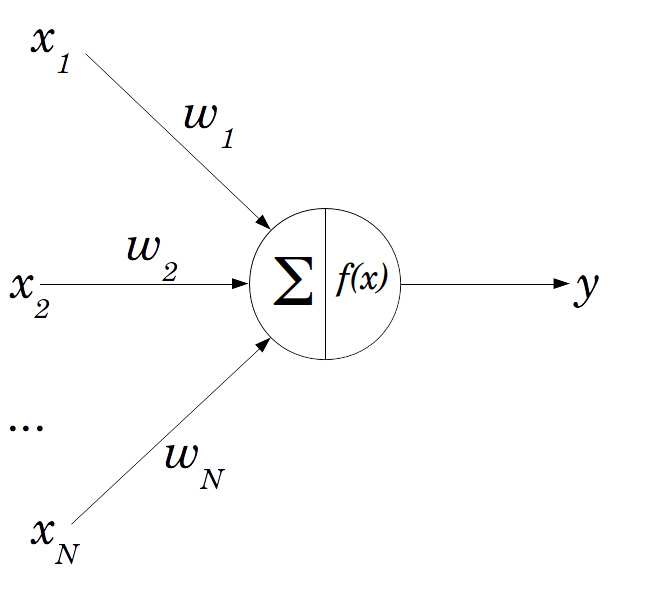
\includegraphics[width=9cm]{Bilder/perceptron.png} 
		\caption[Linear Threshold Unit]{Linear Threshold Unit \cite{PhilippeLucidarme.2017}}
		\label{ltu}
	\end{center}
\end{figure}

Es besteht aus $n$ Eingängen mit $x_{i} \in \mathbb{Q}$, die im Inputvektor $\boldsymbol{x}$ zusammengefasst werden. Jeder Eingang wird mit einem Gewicht $w_{i}$ aus dem Gewichtsvektor $\boldsymbol{w}$ versehen \cite{AurelienGeron.2018}. Die LTU berechnet das Skalarprodukt $\boldsymbol{w}^{T} \circ \boldsymbol{x}$ aller Eingänge $\boldsymbol{x}$ mit ihren Gewichten $\boldsymbol{w}$ und wendet anschließend auf das Ergebnis $z$ eine Aktivierungsfunktion an \cite{AurelienGeron.2018}. Das Ergebnis $h_{w}(x)$ kann anschließend als Eingabe für ein weiteres Perzeptron dienen. Die einfachste Aktivierungsfunkion für ANNs ist die \textit{Heaviside-Funktion} \cite{AurelienGeron.2018}: 

\begin{equation} \label{heaviside}
\begin{split}
h_{w}(x) = s(\boldsymbol{w}^{T} \circ \boldsymbol{x}) = s(z) = \\\ \begin{pmatrix} 
w_{1}&&w_{2}&&\dots&& w_{n}\\ 
\end{pmatrix} 
\circ 
\begin{pmatrix} x_{1}\\
x_{2}\\
\vdots\\
x_{n}\\
\end{pmatrix}) = 
\begin{cases}
1 & \text{wenn} z \geq 0 \\
0 & \text{wenn} z < 0 .\\
\end{cases}
\end{split}
\end{equation}
\equations{Die Heaviside-Funktion}

Falls eine Klassifizierung mit Wahrscheinlichkeiten vorliegen soll, so ist die letzte Schicht eines Perzeptrons meist mit der \textit{Softmax-Funktion}

\begin{equation} \label{softmax}
h_{w}(x) = \sigma(z)_j = \frac{e^{z_j}}{\sum_{i=0}^n e^{z_i} }
\end{equation}
\equations{Die Softmax-Funktion}

implementiert, die den Wert des $j$-ten LTUs einer Schicht mit allen anderen $n$ Werten der LTUs derselben Schicht ins Verhältnis setzt \cite{AurelienGeron.2018}. Es gibt eine Vielzahl an möglichen Aktivierungsfunktionen, die im darauffolgenden Unterkapitel \textit{Hyperparameter} betrachtet werden.


Die Aktivierung einer LTU hängt zusätzlich von einem Schwellwert $\theta$ ab, der durch einen sogenannten \textit{Bias} festgelegt wird. Dies ist die Gewichtung des letzten Eingangs, der standardmäßig den Wert 1 liefert. Wird die Gewichtung negativ gewählt, so ist es schwieriger die LTU zu aktivieren, während eine positive Gewichtung die Aktivierung vereinfacht \cite{AurelienGeron.2018}.

Nun bilden ein oder mehrere Schichten solcher LTUs ein Perzeptron. Jede einzelne LTU ist dabei mit allen LTUs der vorherigen Schicht verbunden (siehe Abbildung \ref{neural_network}) \cite{AurelienGeron.2018}. Hier wird auch von sogenannten vollständig verbundenen Schichten (engl.: \textit{Fully-Connected Layer}) gesprochen. Die beiden LTUs zur Ausgabe können dabei Aussagen über eine Klassifikation von Daten anhand der Eingangsdaten treffen, während die LTUs im Input Layer wesentlich Daten weiter reichen. Die Verbindungen zur ersten Schicht des Hidden Layer sind stets mit Eins belegt. Existiert keine verborgene Schicht, so wird das ANN als einschichtiges Perzeptron bezeichnet, ab einer oder mehr verborgenen Schichten wird bereits von einem \textit{Multi-Layer Perzeptron} (MLP), einem mehrschichtigen Perzeptron, gesprochen \cite{AurelienGeron.2018}. Ist das neuronale Netz optimal trainiert, so ist am Ende nur eines der LTUs zur Ausgabe aktiviert. Das folgende ANN ist zudem ein Beispiel für ein sogenanntes \textit{Feed Forward Network}, bei dem die Auswertung der Daten von einer Schicht zur nächsten weitergereicht wird, ohne zu bereits besuchten Schichte zurückzukehren \cite{AurelienGeron.2018}.

\begin{figure}[ht]
	\begin{center}
		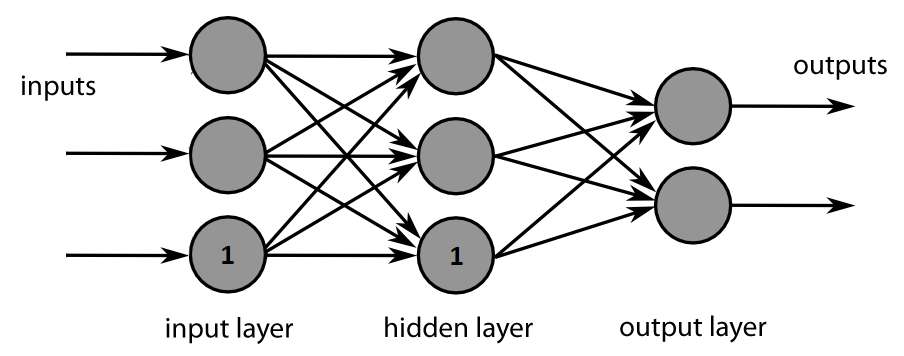
\includegraphics[width=12cm]{Bilder/neural_network.png} 
		\caption[Das einschichtige Perzeptron]{Das einschichtige Perzeptron \cite{Wikipedia.20190123}}
		\label{neural_network}
	\end{center}
\end{figure}

\subsection*{Lernmethoden}

Im Wesentlichen existieren vier Methoden, mit deren Hilfe neuronale Netze trainiert werden können. Beim \textit{überwachten Lernen} werden den Trainingsdaten Lösungen, sogenannte \textit{Labels}, hinzugefügt. Klassifikationsprobleme stellen eine typische Problemstellung für überwachte Lernverfahren dar. Auch die später eingeführten Objektdetektoren werden mittels überwachtem Lernen trainiert \cite{AurelienGeron.2018}. 

Beim \textit{unüberwachten Lernen} werden den Trainingsdaten keinerlei Lösungen hinzugefügt, der Algorithmus muss selbstständig Klassifikationsaussagen treffen können. Ein Beispiel hierzu wäre \textit{K-Means Clustering} \cite{AurelienGeron.2018}. 

\textit{Deep Belief Networks} (DBNs) bestehend aus einzelnen \textit{Restricted Boltzmann Machines} (RBMs) werden zunächst unüberwacht trainiert, bevor im \textit{Fine Tuning} das Gesamtnetzwerk mit überwachten Lerntechniken fertiggestellt wird. Es wird hier von \textit{halbüberwachtem Lernen} gesprochen.

Als letztes ist das sogenannte \textit{Reinforcement Learning} zu nennen. Hierbei wird ein neuronales Netz durch das Erteilen von Belohnungen bzw. Bestrafungen so konditioniert, dass es zukünftig basierend auf der wahrgenommenen Umwelt selbstsicher richtige Aktionen auswählen kann.

\subsection*{Gradientenverfahren und Backpropagation}

Um zu verstehen, wie ein neuronales Netz durch überwachtes Lernen \glqq lernt\grqq{}, muss zunächst der Begriff der Kostenfunktion (engl.: \textit{cost function}) eingeführt werden. Die Kostenfunktion ist ein Qualitätsmaß dafür, wie weit die Ausgabe einer LTU vom erwarteten Wert abweicht \cite{AurelienGeron.2018}. Angenommen dem neuronalen Netz wird ein Datensatz zur Klassifikation übergeben, so ist am Ende meist nicht nur eine LTU zu Ausgabe aktiviert, was auf eine eindeutige Klassifikation schließen würde, sondern meist mehrere zu einem frühen Stadium des neuronalen Netzes.

Eine oft genutzte Kostenfunktion ist die \textit{Root Mean Squared Error Funktion} (RMSE) \cite{AurelienGeron.2018}:

\begin{equation} \label{mse}
E(\boldsymbol{z},\boldsymbol{o}) = \sqrt{\frac{1}{n}\sum_{k=0}^n \lVert{z_k-o_k}\rVert^2} = \sqrt{\frac{1}{n}\sum_{k=0}^n (z_k-o_k)^2}.
\end{equation}
\equations{Die RMSE-Funktion}

Hierbei ist $z$ der erwartete Ausgabevektor des Perzeptrons beim überwachten Lernen, während $o$ die momentane Ausgabe darstellt. Den Fehler der Abweichung dieser beiden Werte gilt es nun schrittweise zu minimieren. Um dies zu erreichen können die drei Parameter

\begin{enumerate}
	\item Gewichtung der Verbindungen zum Perzeptron
	\item Bias zur Aktivierung der LTUs des Perzeptrons und
	\item Stärke der Aktivierung des vorherigen Perzeptrons
\end{enumerate}

angepasst werden \cite{AurelienGeron.2018}. Hierbei wird das sogenannte \textit{Gradientenverfahren} eingesetzt. Es berechnet in einem iterativen Prozess über mehrere Testdaten das globale Minimum der Kostenfunktion nach den Gewichtungen der Verbindungen und damit auch nach den Bias Werten, die natürlich ebenso Gewichtungen darstellen. Ergebnis eines Durchlaufs im Gradientenverfahren (\ref{gradientenverfahren}) ist die Gewichtungsmatrix, die die Änderung der Gewichtung jeder einzelnen Verbindung eines Perzeptrons zu jeder LTU des Folgeperzeptrons angibt \cite{AurelienGeron.2018}:

\begin{equation} \label{gradientenverfahren}
w_{ijt} = w_{ijt-1} - \eta\frac{\partial E}{\partial w_{ij}}. \qquad\text{\cite{PhilippeLucidarme.2017}} 
\end{equation}
\equations{Neuberechnung der Gewichtungsmatrix durch partielle Differentiation}

Das Gradientenverfahren eignet sich allerdings nur für stetig differenzierbare Funktionen ohne Plateaus. Somit können beispielsweise bei der Heaviside-Funktion als Aktivierungsfunktion Probleme auftreten, da eine Ableitung der Kostenfunktion stets Null betragen würde, wohingegen bei der später eingeführten Sigmoid-Funktion im gesamten Definitionsbereich immer kleine Änderung der Gewichtungen zu verzeichnen wären \cite{AurelienGeron.2018}.

Nun stellt sich auch der Vorteil von MSE als Kostenfunktion gegenüber anderen, durchaus komplexeren Kostenfunktionen heraus. Während MSE genau ein Minimum, das zugleich das globale Minimum der Funktion darstellt, besitzt, haben andere Kostenfunktionen im Gradientenverfahren das Problem, dass anstelle des globalen Minimums auch nur lokale Minima erreicht werden können \cite{AurelienGeron.2018}. Dies hat zur Folge, dass mehrere iterative Durchlaufe mit mehreren Testdatensätzen nötig werden, um durch unterschiedliche Startkonfigurationen die unterschiedlichen Minima miteinander vergleichen zu können und damit das globale Minimum herauszustellen.

Durch das Gradientenverfahren werden somit nur diejenigen Verbindungen verstärkt, die zum richtigen Ergebnis führen. 

Nun bleibt nur noch die dritte Möglichkeit zur Minimierung der Kostenfunktion übrig, die Anpassung der Stärke der Aktivierung des vorherigen Perzeptrons. Zu diesem Problem veröffentlichten David E. Rumelhart, Geoffrey E. Hinton und Ronald J. Williams 1985 den sogenannten \textit{Backpropagation-Algorithmus} \cite{DavidE.Rumelhart.September1985}. Dieser berechnet mit Hilfe des Gradientenverfahren welchen Anteil am Fehler der Ausgabe jede LTU des letzten Perzeptrons hat und anschließend welcher Anteil davon wiederum auf das vorherige Perzeptron der vergorenen Schicht zurück zu führen ist. Das Gradientenverfahren wird solange wiederholt, bis die Eingangsschicht erreicht wurde, es berechnet also für jede LTU deren Anteil am Fehler des Ergebnisses \cite{AurelienGeron.2018}.

Mit Hilfe des Gradientenverfahren im Backpropagation Algorithmus wird nun also das neuronale Netz durch mehrere iterative Durchläufe trainiert, wobei das Training als Anpassung der Gewichtungen einzelner Verbindungen zu verstehen ist.